\documentclass[a4paper,11pt]{article}

\usepackage[utf8]{inputenc}

\usepackage{minted}

\usepackage{graphicx}

\begin{document}

\title{
    \textbf{Double Linked Lists}
}
\author{Ruxandra-Stefania Tudose}
\date{Fall 2023}

\maketitle

\section*{Introduction}

This report aims to open a window on an 'updated' linked list, which includes several new features, among which the ability of
traversing the data structure both forward and backwards. 
Therefore, the double linked list consists of an extra field in the cell, which always keeps track of the previous neighbour. The main focus
of this experiment are the two new operations, namely \textit{unlink} and \textit{insert}, but most importantly how they behave depending on the 
type of the linked list and their sizes.


\section*{Implementing a double linked list: the methods}

In order to create the double linked list, the starting point was my implementaion of the simple linked list.
In other words, I first added the new \textbf{previous} node and then,
the only methods that had to be adapted were the \textit{remove} and \textit{asArray} methods. The second method, \textit{asArray}, is a method I 
created in order to debug and see the changes to the list after having called any of the methods.
Having said that, below there are the parts of the \textit{remove} method that have been changed for the double linked list, which 
include connecting the references of all nodes to the
to previous ones as well.

\begin{minted}{java}
        // code for special case - remove first element
        if(previous.number == item) { 
            first = first.next;
            first.prev = null; //extra for double linked list
        }    
   
        while (current.next != null) {
            if(current.number == item) {
                previous.next = current.next;
                current.next.prev = previous; //extra for double linked list
            }

        //updating the references in order to move forward in the list
            previous = current;
            current = current.next;
        }
\end{minted}  


\subsection*{My approach: Checking accuracy first}

As far as my approach is concerned, before moving on with the assignement, the next step was to check the accuracy of the new code upgrades.
Therefore, in order to make sure that the previous cells are also connected, I navigated the list both forward and backwards 
using the 'length' method and displayed the size, which as expected was double to the real one. After I made sure it was working correctly , I commented
these extra lines of code included below: \newline\newline

\begin{minted}{java}
//navigating the double linked list backwards and incrementing 'count'
    while(index.prev != null) {
        count ++; //variable that keeps track of the list's size
        index = index.prev;
    }

    return count + 2; //'+2' to count the ends of the list

\end{minted}

\section*{Setting up the \textit{unlink} and \textit{insert} methods}

While the \textit{insert} is pretty similar in both cases, it is shorter for the simple linked list since the only thing we have to do is 
to connect the new node and upgrade the head of the whole data structure. 

\begin{minted}{java}

    void insert (Node toAdd) {

        toAdd.next = first; //linking the new node
        first = toAdd; //updating the head of the list
    }

\end{minted}

On the other hand, as far as the double linked list is concerned, more operations have to be executed since there are more fields that have to be linked,
as presented below:

\begin{minted}{java}
   
    void insert (Node toAdd) {
        toAdd.next = first; //connecting the node to the list
        toAdd.prev = null; //setting the prev field
        first.prev = toAdd;//updating the prev field of the initial list head
        first = toAdd; //updating the head of the list
    }
\end{minted}

\textit{Note: }When writing these operations it is highly important to keep track of the order they are executed in, as they are not symmetrical.
And what do I mean by that is for instance, the head of the list
should not be updated before the linking with the new node is done. If done this way, the reference of the whole list is lost, which is something to be 
avoided! Therefore, the order matters! \newline

As far as the unlink method is concerned, there are several differences between the two lists, however, the main one is that regardless of having the reference
of the new node, in the simple linked list we still have to traverse all the way through in order to properly identify and remove it. Conversely, the node
of the doubly linked list gives us all necessary pieces of information, the only thing being left is to make the correct linking.
That is precisely why this operation's time complexity is \textit{O(1)}, while the simple linked list's is \textit{O(n)}. \newline

In order to better understand the differences between the two, the following table has been created:

\begin{table}[h!]
    \centering
    \begin{tabular}{||c c c||} 
    \hline
    Type & unlink & insert\\ [0.5ex]
    \hline
    LinkedDouble& O(1) & O(1) \\
    LinkedSimple & O(n) & O(1) \\ [1ex] 
    \hline
    \end{tabular}
    \caption{Time complexity analysis of the \textit{unlink} and \textit{insert} operations.} 
    \label{table:1}
\end{table}


\section*{Unlinking and inserting nodes}

After having set up the methods, the next step was identifying the difference in the execution time when unlinking and inserting a node 
in both lists. From the perspective of relevance, this comparison has been done taking into consideration \textit{the ratio} between the simple 
and double linked list execution time. 

Although the nodes which were unlinked and then inserted were generated randomly,
in order for the results to be \textit{relevant} (especially because we have to go through the whole simple linked list for the unlink operation),
the two operations were executed using the same node in both data structures. \newline

As it can be noticed from the table below, at first, namely for the small lists, the unlink and insert operations are executed much faster, fact which does make sense: there are fewer lines of code that have to be executed in the \textit{insert} method, which does make up for the time lost in the \textit{unlink} method (it should be taken into consideration that the lists are not very long). \newline\newline
However, as the 
array grows, the advantages of the double linked list make their presence felt. In other words, since both insert operations are \textit{O(1)}, 
the difference in the time execution between the two \textit{(which can be seen in the growing value of the ratio) }is given by the \textit{unlink} operation.\newline \newline
And that is simply because the simple linked list has to be traversed all the way in order to add the new node. Unlike the double linked list, the operation here is not instantaneous.


\begin{table}[h!]
    \centering
    \begin{tabular}{||c c||} 
    \hline
     n & simply/doubly ratio \\ [0.5ex]
    \hline
    25 & 0.4 \\
    50 & 0.6 \\
    100 & 0.9 \\
    400 & 1.17 \\
    1600 & 1.6 \\
    3200 & 2.5 \\
    6400 & 1.6 \\
    12800 & 1.9 \\
    25600 & 2 \\
    52000 & 1.9 \\[1ex]
    \hline
    \end{tabular}
    \caption{The ratio evolution between the simple linked list and double linked list.} 
    \label{table:2}
\end{table}

\begin{figure}[ht]
    \centering
    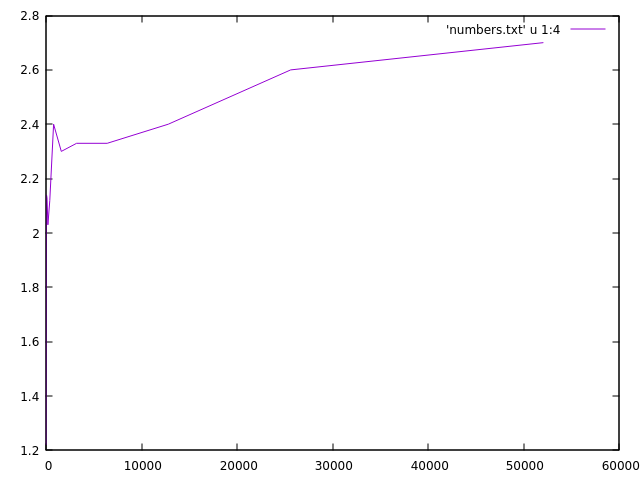
\includegraphics[width=0.6\textwidth]{doubly_simply_ratio.png}
    \caption{The graph describing the evolution of the ratio between the doubly and simply linked lists.}
    \label{fig:1}
\end{figure} 
  

To put it briefly, the graph below illustrates the ratio evolution between the two data structures and what is of particular interest is the way the ratio actually stabilises as the sizes of the linked lists increase. We can, therefore, conclude that for large data sets, \textit{unlinking} a node in a double linked list is highly efficient compared to a single linked list! \newline

\textit{Note: } Since the references that are to be unlinked are randomly generated, it is most likely that the spike in the graph below was generated because the node that was removed was at the end of the linked lists. Therefore, the execution time of the simple linked list increased, which in turn made the ratio grow as well.

\section*{Difficulties} 

The main difficulty I encountered in this assignment was to always keep track of all the connections
that I had to set up when unlinking or inserting a node, especially when it comes to the 
double linked list. For instance, at some point I kept getting an error and that was because I had forgotten to upgrade the new head of the list.

\section*{Conclusion}

All in all, setting up a double linked list requires an organised approach and a lot of attention mostly when creating the node connections. However, once everything runs smoothly, it does pay off! And that is especially when removing a node from the whole data structure!
\end{document}